\section{Circuits}
\label{sec:circuits}

\begin{sessioncard}
\textbf{Session 7.} \emph{Goal:} see how single components combine into an algorithm, on two examples: a
mechanism by which a model continues a repeated pattern, and the mechanism behind the running example.
\emph{Experiments:} GPT-2 small on repeated random text (\cref{exp:repeat}), finding the heads that do it
(\cref{exp:inductionheads}), and removing them (\cref{exp:inductionablate}).
\emph{Prerequisites:} sessions 2 and 6.
\end{sessioncard}

The tools of the last sessions tell us what is represented and which components matter. A \emph{circuit} is an
answer to the remaining question: how the components work together. The term was coined in the study of vision
models \citep{olah2020zoom}.

\subsection{What counts as a circuit}

By the argument of \cref{prop:sum}, the input of every component is a sum of the outputs of earlier components.
We can therefore draw the model as a graph. The nodes are the embeddings, the attention heads and the MLPs, and
there is an edge from every component to every later one. This graph is the same for every model of the same
architecture. What differs is which edges carry something that matters.

\begin{definition}[Circuit]\label{def:circuit}
A \emph{circuit} for a task is a subgraph of this graph together with a description of what each of its nodes
computes on the task.
\end{definition}

A drawing of nodes and arrows is easy to produce, so the definition is only useful together with tests.
\citet{wang2023interpretability} proposed three. In all of them, components outside the set under study are
replaced by their mean over a reference set of prompts (mean ablation, session 6).
\begin{itemize}
\item \textbf{Faithfulness.} The circuit alone, with everything else ablated, performs about as well as the
full model.
\item \textbf{Completeness.} The circuit contains all components that take part in the behaviour, including
those that would only step in if others failed.
\item \textbf{Minimality.} Every node of the circuit is needed.
\end{itemize}

\subsection{Induction: continuing a repeated pattern}
\label{sec:induction}

Text is full of repetitions. If the sequence \tok{[A][B]} has occurred and the token \tok{[A]} occurs again,
then \tok{[B]} is a good guess for the next token. Models learn this rule early, and the mechanism that
implements it was the first algorithm found inside a transformer \citep{elhage2021mathematical}.

\begin{experiment}[A model can repeat what it has never seen]\label{exp:repeat} \script{exp\_induction.py}
We give GPT-2 small a sequence of $40$ random tokens followed by the same $40$ tokens again. Random tokens form
text that the model has never seen, so nothing it has memorised can help. \Cref{fig:inductionloss} (left) shows
the loss on the next token at every position, averaged over $20$ such sequences. In the first copy the loss is
$13.2$, worse than the value $10.8$ of a uniform guess over the vocabulary. Inside the second copy it is
$0.28$. The model predicts each token of the second copy almost perfectly, and the only source of
this information is the first copy.
\end{experiment}

\begin{figure}[t]
\centering
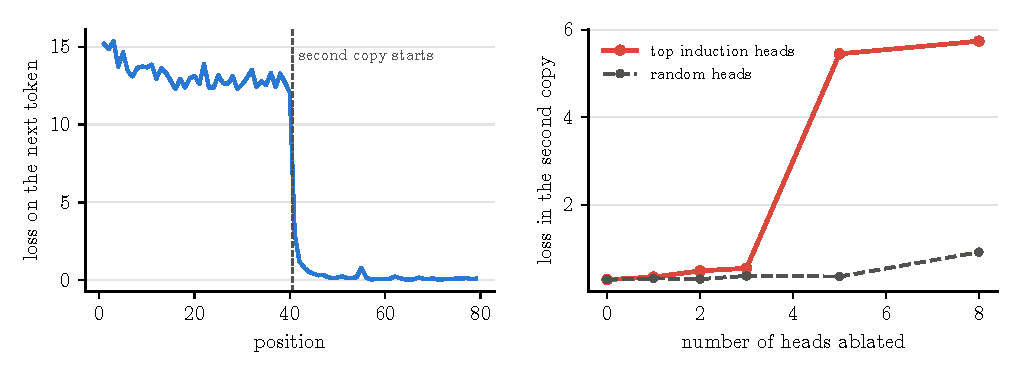
\includegraphics[width=0.95\textwidth]{figures/fig_induction_loss.pdf}
\caption{GPT-2 small on $40$ random tokens that are repeated once. Left: loss on the next token at each position
(\cref{exp:repeat}). Right: loss in the second copy when the output of some heads is replaced by its mean
(\cref{exp:inductionablate}).}
\label{fig:inductionloss}
\end{figure}

How can a transformer do this? The task needs, at the second \tok{[A]}, to find the earlier \tok{[A]} and look
one step to its right. A single attention head cannot ask for ``the position after a token equal to mine'',
because the score in \eqref{eq:pattern} compares the destination with the source itself. Two heads in different
layers can (\cref{fig:induction}).

\begin{enumerate}
\item A \emph{previous-token head} in an early layer attends from every position to the position before it.
At the position of \tok{[B]} it writes into the stream the information ``the token before me was \tok{[A]}''.
We have seen such a head in \cref{exp:attention}.
\item An \emph{induction head} in a later layer sits at the second occurrence of \tok{[A]}. It asks for
positions whose stream says ``the token before me was \tok{[A]}''. Thanks to the first head, this description
fits the position of \tok{[B]}, and the head attends there.
\item The matrix $W_{OV}$ of the induction head copies: it raises the logit of the token that it attends to. The
model predicts \tok{[B]}.
\end{enumerate}
The second head reads what the first one wrote. This is the simplest example of \emph{composition}, the use of
the output of one head by another, and it is where algorithms begin.

\begin{figure}[t]
\centering
\begin{tikzpicture}[>=Latex, font=\small, tokn/.style={draw=tutgrey, fill=tutpaper, minimum height=6mm, minimum width=9mm}]
\node (l) at (0,0) {$\cdots$};
\node[tokn] (a1) at (1.3,0) {\tok{[A]}};
\node[tokn] (b1) at (2.7,0) {\tok{[B]}};
\node (m) at (4.6,0) {$\cdots$};
\node[tokn] (a2) at (6.5,0) {\tok{[A]}};
\node[tokn, dashed, fill=white] (b2) at (7.9,0) {\tok{[B]}};
\draw[->, line width=1pt, tutblue] (a1.south) to[out=-60,in=-120] node[below, text=black, align=center]
  {(1) previous-token head, early layer:\\ ``the token before me was \tok{[A]}''} (b1.south);
\draw[->, line width=1pt, tutred] (b1.north) to[out=50,in=130] node[above, text=black, align=center]
  {(2) induction head, later layer: attends to the token that follows an earlier \tok{[A]}} (a2.north);
\draw[->, line width=1pt, tutred] (a2.east) -- node[below=3mm, text=black, align=center, xshift=14mm] {(3) copies \tok{[B]}\\ to the prediction} (b2.west);
\end{tikzpicture}
\caption{The induction circuit. Arrows show the flow of information from a source position to a destination
position. The dashed box is the predicted next token.}
\label{fig:induction}
\end{figure}

\begin{experiment}[Finding the heads]\label{exp:inductionheads} \script{exp\_induction.py}
The mechanism makes a prediction that we can check on the patterns alone. An induction head at a position of the
second copy should attend to the token \emph{after} the earlier occurrence of the current token, which is $39$
positions back. For every head we average the attention weight on that position (\cref{fig:inductionheads},
left). Five heads stand out with scores above $0.8$: 5.5, 6.9, 7.10, 5.1 and 7.2. The right panel shows the
pattern of head 5.5 on one sequence. In the first copy it rests on the start token. In the second copy it forms
a sharp diagonal stripe, shifted by one position from the earlier copy.

The same data contain the other ingredients. The heads that attend most to the previous position are 4.11, with
an average weight of $0.99$, and 3.7, 6.8 and 2.2. The heads that attend to the earlier occurrence of the
current token itself, called \emph{duplicate token heads}, are 3.0 and 0.5.
\end{experiment}

\begin{figure}[t]
\centering
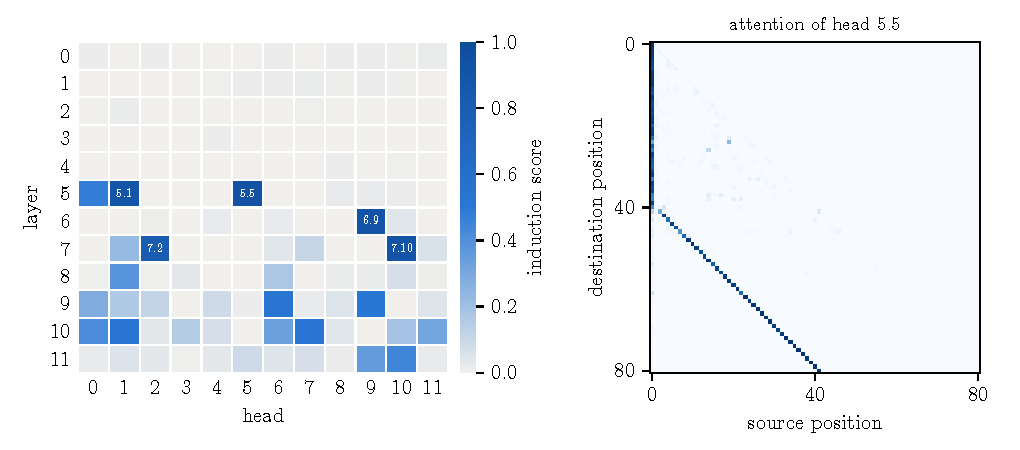
\includegraphics[width=0.95\textwidth]{figures/fig_induction_heads.pdf}
\caption{Left: induction score of every head of GPT-2 small, the average attention from a token of the second
copy to the token after its earlier occurrence (\cref{exp:inductionheads}). Right: attention pattern of head 5.5
on one sequence of $81$ tokens. Position $0$ is the start token.}
\label{fig:inductionheads}
\end{figure}

\begin{experiment}[Removing the heads]\label{exp:inductionablate} \script{exp\_induction.py}
The scores are observations. To test whether these heads are responsible for the behaviour, we take the heads
with the highest induction scores and replace the output of each by its mean over all positions of the same $20$
sequences. Then we measure the loss in the second copy (\cref{fig:inductionloss}, right). Without ablation the
loss is $0.28$. With the best head ablated it is $0.34$, with the best three it is $0.55$, with the best four it
is $3.5$, and with the best five it is $5.4$. Ablating the same numbers of randomly chosen heads gives at most
$0.76$, on average over five draws.

Two conclusions follow. These five heads carry the behaviour. And they do so redundantly: when the best three
are removed, the remaining two, 5.1 and 7.2, still keep the loss at $0.55$. An ablation of one head at a time
would have concluded that no single head matters, which is Lesson 2 of session 6 once more.
\end{experiment}

Induction heads are not a curiosity of one model. \citet{olsson2022context} found them in models of many sizes
and showed that they form during a short window early in training, at the same time as the ability of the model
to use its context improves sharply. They are a mechanism of \emph{in-context learning}: the model picks up a
pattern from the prompt and continues it.

\subsection{The circuit of the running example}
\label{sec:ioi}

We can now assemble what sessions 2 and 6 found about the IOI task into the circuit of
\citet{wang2023interpretability}, shown in \cref{fig:ioi}. As in their paper, we work backwards from the output.

\paragraph{Who writes the answer?} The name mover heads 9.9, 9.6 and 10.0. At the last position they attend to
the indirect object (\cref{exp:attention}) and write in the direction that raises its logit (\cref{exp:dla}).
Their $W_{OV}$ copies the name that they attend to.

\paragraph{Why do they attend to the right name?} Both names are candidates. The name movers avoid the subject
because of the S-inhibition heads 7.3, 7.9, 8.6 and 8.10. These heads sit at the last position and attend to
S2. They write a signal into the last position that changes what the name movers ask for, so that positions
holding the subject receive less attention. This is the transfer from S2 to the last position in layers 7 and 8
that we saw in \cref{exp:residpatch}. It also explains why these heads have a large patching effect and almost
no direct effect in \cref{tab:heads}.

\paragraph{How do the S-inhibition heads know which name is repeated?} Two groups of heads at S2 detect the
repetition, and we have just met both. The duplicate token heads, among them 3.0, attend from S2 to the earlier
occurrence S1 of the same token. The induction heads, among them 5.5 and 6.9, attend from S2 to the token
\emph{after} S1, using the output of the previous-token heads 2.2 and 4.11 exactly as in \cref{sec:induction}.
Both groups write to the stream at S2 that this token has occurred before, and the S-inhibition heads read it.
Several of the heads that \cref{exp:inductionheads} found on random tokens, namely 5.5, 6.9, 3.0, 4.11 and 2.2,
are the ones that do this job in an English sentence.

\begin{figure}[t]
\centering
\begin{tikzpicture}[>=Latex, font=\footnotesize,
  tokn/.style={draw=tutgrey, fill=tutpaper, minimum height=5.5mm, inner sep=3pt},
  cls/.style={draw=tutgrey, rounded corners=2pt, align=center, inner sep=3.5pt, fill=#1}, cls/.default=tutblue!10]
\node[tokn] (t1) at (0,0) {\tok{When}};
\node[tokn] (io) at (1.4,0) {\tok{Mary}};
\node[tokn] (t3) at (2.6,0) {\tok{and}};
\node[tokn] (s1) at (3.8,0) {\tok{John}};
\node[tokn] (s1p) at (5.1,0) {\tok{went}};
\node (d1) at (6.3,0) {$\cdots$};
\node[tokn] (s2) at (7.7,0) {\tok{John}};
\node (d2) at (9.4,0) {$\cdots$};
\node[tokn] (end) at (11.2,0) {\tok{to}};
\node[below=1pt of io, tutgrey] {IO};
\node[below=1pt of s1, tutgrey] {S1};
\node[below=1pt of s2, tutgrey] {S2};
\node[below=1pt of end, tutgrey] {last position};
\node[cls] (prev) at (5.1,2.2) {previous token\\ 2.2, 4.11};
\node[cls] (dup) at (7.7,1.05) {duplicate token\\ 0.1, 3.0};
\node[cls] (ind) at (7.7,2.2) {induction\\ 5.5, 6.9};
\node[cls] (sinh) at (11.2,3.3) {S-inhibition\\ 7.3, 7.9, 8.6, 8.10};
\node[cls=tutred!12] (nm) at (9.3,5.3) {name movers\\ 9.9, 9.6, 10.0};
\node[cls=tutblue!22] (neg) at (13.0,5.3) {negative name movers\\ 10.7, 11.10};
\node (out) at (11.2,6.9) {logit difference in favour of \tok{Mary}};
\node at (4.7,5.6) {copy the attended name};
\draw[->, tutgrey] (s1.north) -- (prev.south west);
\draw[->, tutgrey] (s1.north east) -- (dup.west);
\draw[->, tutgrey] (prev.east) -- (ind.west);
\draw[->, tutgrey] (dup.east) to[out=0,in=200] (sinh.south west);
\draw[->, tutgrey] (ind.east) to[out=0,in=180] (sinh.west);
\draw[->, tutgrey] (sinh.north) to[out=120,in=-50] node[right=2pt, pos=0.5, text=black] {avoid S} (nm.south east);
\draw[->, tutred, line width=0.9pt] (io.north) to[out=80,in=180] (nm.west);
\draw[->, tutred, line width=0.9pt] (nm.north) -- node[left=2pt, text=black] {$+$} (out.south west);
\draw[->, tutblue, line width=0.9pt] (neg.north) -- node[right=2pt, text=black] {$-$} (out.south east);
\end{tikzpicture}
\caption{The circuit for indirect object identification in GPT-2 small, simplified from
\citet{wang2023interpretability}. Each box is a class of attention heads with its main members, drawn above the position at which
the heads write. Arrows show the flow of information. The backup name movers are omitted.}
\label{fig:ioi}
\end{figure}

\paragraph{The algorithm.} In words, the model does three things. It finds the name that occurs twice. It
tells the last position to ignore that name. It copies the name that is left. Two further classes complicate
the picture. The negative name movers 10.7 and 11.10 attend to the same name as the name movers and write
\emph{against} it, and the backup name movers become active when the name movers are removed. We saw the trace
of both in \cref{exp:lens,exp:headpatch}.

\paragraph{How good is the explanation?} The circuit of \citet{wang2023interpretability} has 26 heads in seven
classes. On their set of prompts the full model has an average logit difference of $3.56$. With every head
outside the circuit mean-ablated, the circuit retains $87\%$ of that value. This is a strong result, and it also
marks the limits of the best-understood circuit in a real language model. It concerns one narrow task on
sentences that follow a template. A part of the behaviour remains unexplained. Two classes of heads, the
negative and the backup name movers, are described without a clear account of why training produced them. And
the role of the MLPs is left open.

\begin{caution}
Our own experiments on 12 prompts reproduce the signatures of the heads that act at S2 and at the last
position. They say nothing about the heads that act earlier: the clean and the corrupted prompt agree before S2,
so the previous-token heads behave identically in both runs and cannot show up in our patching experiment. Our
experiments are also not a validation of the circuit. We did not run path patching, and we did not test
faithfulness, completeness or minimality.
\end{caution}

\begin{takeaways}
A circuit is a subgraph of components with a description of what each one computes, and it has to be tested for
faithfulness, completeness and minimality. The induction circuit combines a previous-token head and an induction
head. In GPT-2 small five induction heads carry the ability to continue a repeated sequence, redundantly. The
circuit of the running example reuses the same kinds of heads: it finds the repeated name, tells the last
position to avoid it, and copies the other name.
\end{takeaways}

\subsection*{Questions for the seminar}

\begin{exercise}[Why induction needs two layers]\label{ex:induction}
Explain why the induction mechanism cannot be implemented by a transformer with a single layer. Use the fact
that, in the first layer, the stream at a position contains only the token at that position and the position
itself.
\end{exercise}

\begin{exercise}[Faithful and still incomplete]\label{ex:redundant}
A model solves a task with two heads that do the same job, so that the task is solved as long as at least one of
them works. A colleague proposes the circuit that consists of the first head alone. Evaluate the faithfulness,
the completeness and the minimality of this circuit. Which experiment of this session shows such redundancy,
and which class of heads of the IOI task plays the role of the second head?
\end{exercise}

\begin{exercise}[Eighty-seven per cent]\label{ex:eightyseven}
The IOI circuit retains $87\%$ of the logit difference when all other heads are mean-ablated. (a) Give two
different explanations of where the remaining $13\%$ could come from. (b) The reference prompts for the mean
ablation are sentences with three unrelated names, none of which is repeated. What would change, and why, if
the means were taken over the IOI prompts themselves? (c) Could a circuit reach $100\%$ and still be a poor
explanation?
\end{exercise}

\begin{exercise}[A prediction]\label{ex:prediction}
The description of the IOI circuit predicts what happens on the prompt \tok{When Mary and John went to the
store, Mary gave a drink to}. It also suggests what should happen on a prompt with three names, such as
\tok{When Mary, John and Paul went to the store, John gave a drink to}. Derive both predictions. How would we
test the second one, and what would we conclude if it failed?
\end{exercise}

\begin{readinglist}
\item \citet{wang2023interpretability}, \emph{ICLR}. The IOI circuit. It remains the model of how to argue for a
circuit.
\item \citet{conmy2023towards}, \emph{NeurIPS}. Automates the search for circuits by removing, one after the
other, all edges whose removal changes the output only a little.
\item \citet{merullo2024circuit}, \emph{ICLR}. Finds that most components of the IOI circuit are used again in a
different task, which is evidence that circuits are built from reusable parts.
\item \citet{singh2024needs}, \emph{ICML}. An experimental study of how induction heads form during training.
\item The original accounts of induction heads, \citet{elhage2021mathematical} and \citet{olsson2022context},
are not peer reviewed. The first is the source of the view of the transformer used in these notes.
\end{readinglist}
